\section{Electronics}

The MVT data acquisition system is designed to readout 6,000 channels of the forward station and 18,000 channels of the
barrel station. With the physics background as high as 20~MHz, the strip hit rates are about 60~kHz and 20~kHz in the
forward detectors and in the barrel detectors, respectively. The readout system is compliant with the CLAS12 requirements
of a 20~kHz maximum trigger rate and provides a sufficiently long data pipeline to cope with up to 16~$\mu$s trigger decision
latency. Timing precision of a few ns is sufficient to limit the number of ghost hits compatible with the timing of the trigger
signals. A charge measurement with a 10-bit dynamic range is enough to cover the full span of the Micromegas detector signals
and to discriminate accurately minimum-ionizing particles (MIPs) from noise. Note that the FT-Trk uses the same readout electronics and architecture as the MVT.

\subsection{Readout System Architecture}

The extremely compact and dense design of the CLAS12 Central Detector leaves a very narrow space between the MVT and
its neighbor subsystems, as well as between the Micromegas detectors themselves.  In addition to the stringent space limitations, the
operational conditions of the tracker are harsh in terms of radiation and the high 5~T magnetic field. The low material budget
is an obvious concern. Consequently, a readout architecture based on off-detector front-end electronics has been adopted.
Lightweight micro-coaxial cable assemblies with low 40~pF/m linear capacitance carry bare, unamplified signals to the Front-End
Units (FEU) housed in crates $\sim$1.5--2~m upstream of the detectors. 

\begin{figure*}[htb]
\begin{center}
 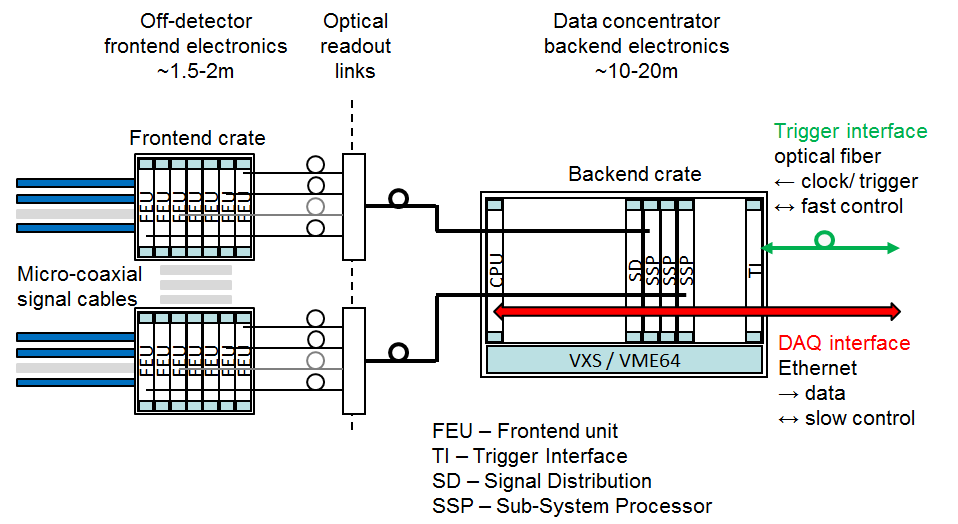
\includegraphics[width=1.6\columnwidth,keepaspectratio]{images/electronics_fig1.png}
\end{center}

 \caption{MVT and FT-Trck readout system.}
 \label{fig:mm-e_1}
\end{figure*}

The front-end electronics are responsible for the amplification and shaping of the detector signals, for holding the latter in a
pipeline waiting for the trigger process to yield, for the digitization and compression of the selected event data, and for their
delivery to the back-end electronics. The back-end is responsible for data concentration event by event. It provides an interface
with the CLAS12 event building system, ensures a fixed latency path between the CLAS12 trigger system~\cite{trigger-nim} 
and the FEUs, and receives the system clock and trigger from the CLAS12 trigger supervisor and synchronously conveys 
them to the FEUs over bidirectional optical links. A schematic representation of the readout system architecture is 
shown in Fig.~\ref{fig:mm-e_1}.

\subsection{The 64-Channel DREAM ASIC}

Depending on the type and size of the CLAS12 Micromegas detectors, the strip capacitances vary from 60 to 120~pF. The total
capacitance seen by the front-end electronics input is even higher, up to 200~pF due to the contribution from the detector
micro-coaxial cables. To achieve a comfortable signal to noise ratio (SNR) well above 10, the equivalent noise charge (ENC) of the
detection chain should be $\sim2500~e^-$ for the $140-200$~pF range of the total input capacitance. At the time of the
detector development, no existing ASICs could deliver the required performance while, in addition, sustain the 20~kHz readout
rate and provide the 16$~\mu$s deep trigger pipeline required. A new 64-channel ASIC, called DREAM (for Dead-timeless
Readout Electronics ASIC for Micromegas), has been developed~\cite{DRM}. 

\begin{figure}[htb]
 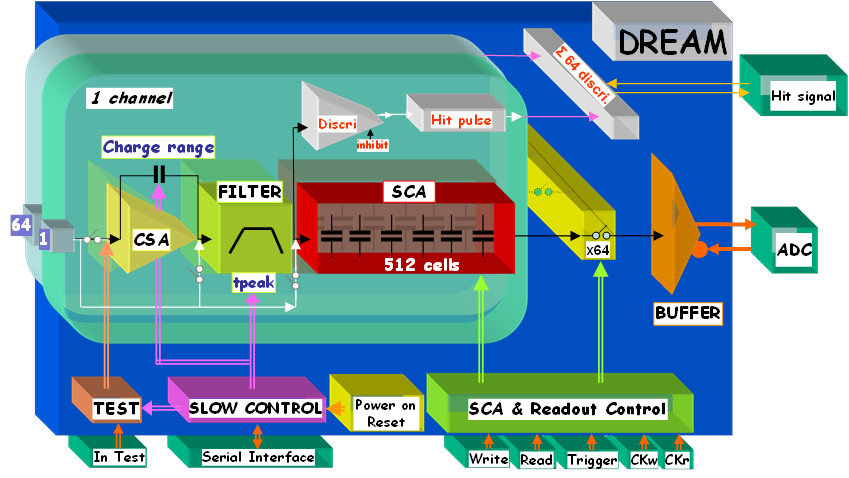
\includegraphics[width=1.0\columnwidth,keepaspectratio]{images/electronics_fig2.png}
 \caption{Block diagram of the DREAM ASIC.}
 \label{fig:mm-e_2}
\end{figure}

The DREAM ASIC block diagram is shown in Fig.~\ref{fig:mm-e_2}. Each channel includes a charge sensitive amplifier 
(CSA) adapted to a wide spread of detector capacitances (up to 1~nF) and
four selectable charge measurement ranges (from 50 to 600~fC), a shaper with programmable peaking times (from 75~ns to
1~$\mu$s), and 512-cell deep Switched Capacitor Array (SCA) used as the trigger pipeline memory and a de-randomization buffer.

The input signals are continuously sampled and stored in the SCA at a rate of up to 50~MHz. Upon reception of the trigger signal,
a programmable number of samples of all channels, corresponding in time to the event, is read out serially through a differential
analog buffer capable of driving an external ADC at a frequency of up to 28~MHz. The sampling is not stopped during the readout
process, which allows nearly dead-timeless operation. Other features, such as the ability to operate with both signal polarities,
the possibility to inject input signals directly into the SCA memory bypassing the filter and/or CSA, and integrated per-channel
discriminators (useful to form trigger primitives), make the chip extremely versatile. The integrated circuit is manufactured in
the AMS CMOS 0.35~$\mu$m technology and is encapsulated in the 128-pin LQFP square package with a 1~mm side and a
0.4~mm pitch.

\subsection{The 512-Channel Front-End Unit (FEU)}

The FEU is a mixed analog-digital electronics board. The analog section comprises eight input connectors, protection circuits,
DREAM ASICs, and an 8-channel flash ADC (see Fig.~\ref{fig:mm-e_3}). The protection circuits are optional.  They are installed
on the FEUs to protect the DREAMs from the sparks of the standard Micromegas detectors. When working with resistive
detectors, the input channels of the DREAM ASICs can be directly connected to the detector strips, improving the signal to
noise ratio. The protected or non-protected type of FEUs are determined during their manufacturing.

\begin{figure}[htb]
 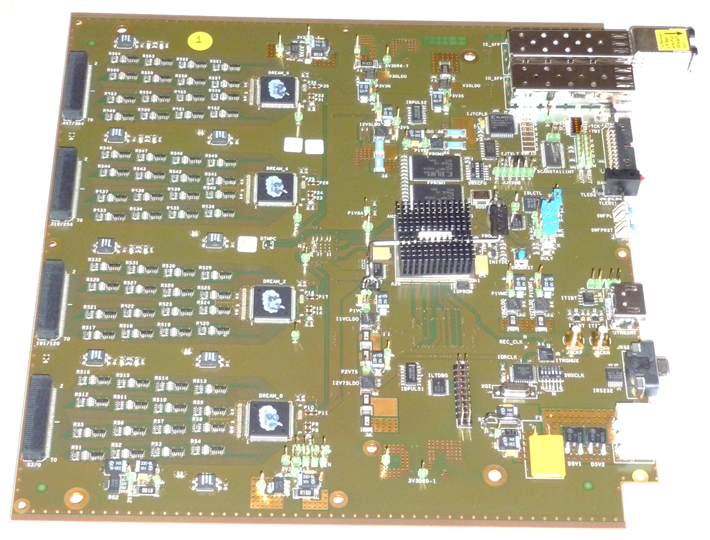
\includegraphics[width=1.0\columnwidth,keepaspectratio]{images/electronics_fig3.png}
 \caption{Photograph of the 512-channel Front-End Unit.}
 \label{fig:mm-e_3}
\end{figure}

As described above, the pre-amplification, shaping, and trigger pipeline functionality is implemented in the DREAM chips. The
analog samples from the eight DREAMs are digitized by an 8-channel 40~MHz 12-bit flash ADC AD9222 from Analog Devices
\cite{ADC}. The eight serial streams of digital data are delivered to the on-board FPGA. The digital section of the board
comprises an xc6vlx75t-2-ff748 FPGA from the Xilinx Virtex-6 device family~\cite{XIL}, its configuration memory, a 2~Mbyte
synchronous SRAM, small form-factor pluggable (SFP) transceivers, an on-board clock synthesizer, and an auxiliary trigger
interface circuit.

The FPGA controls the DREAM integrated circuits and the ADC, producing the sampling and readout clocks, as well as various
required control signals. One of the SFP cages is populated with an optical transceiver module that is used to establish a
synchronous communication channel with the back-end electronics over a 2.5~Gbit/s link. In the downstream direction, the link
encodes the 125~MHz system clock, trigger signals, and fast synchronous commands.

Upon accepting the trigger signal, the FPGA reads the corresponding samples from the DREAMs and optionally applies the
following digital data processing steps. First, after serial to parallel conversion, the pedestals are equalized. Next, for each
sample, the coherent noise affecting the DREAM inputs is estimated and subtracted on a chip-by-chip basis. This greatly
improves the noise immunity of the MVT readout system. Finally, the per-channel zero suppression is performed. The retained
samples describe the signal development in the channel. Fitting their values with a known function allows an accurate estimation of
deposited charge and of signal timing. For each accepted trigger, the FPGA forms an event fragment from the retained channel
data and delivers it to the back-end electronics via the optical channel. The optical channel is also used for setting and monitoring
the run control parameters.

The FEU is a 6U (266~mm) high, 220~mm deep, and 5HP (25.4~mm) wide module. The thickness of its 12-layer PCB is 1.6~mm. It
can be powered from either a 4.3~V or 5~V source and consumes slightly less than 20~W when all eight DREAMs operate in their
most power-hungry mode. The FEUs have been operated in a magnetic field of up to 1.5~T without any perceptible change of their
power consumption or functionality.

\subsection{The Back-End Unit (BEU)}

The back-end of the data acquisition system of the MVT is based on the JLab standard VME/VXS hardware including a trigger
interface (TI), a signal distribution (SD) and a sub-system processor (SSP) board, and a crate controller single board computer
(SBC)~\cite{daq-nim}. The flow of the trigger, data, and control messages is shown in Fig.~\ref{fig:mm-e_4}. 

\begin{figure*}[htb]
\begin{center}
 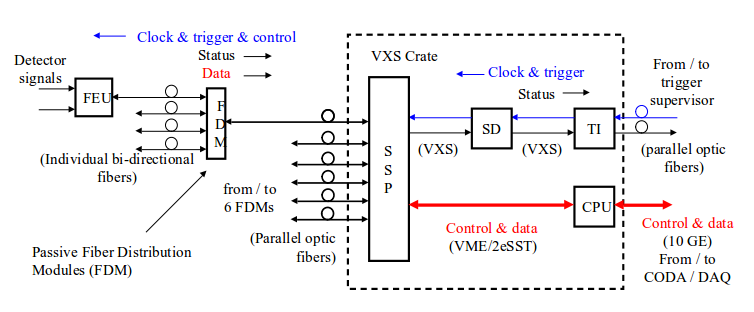
\includegraphics[width=1.6\columnwidth,keepaspectratio]{images/electronics_fig4.png}
\end{center}

 \caption{MVT back-end unit and dataflow.}
 \label{fig:mm-e_4}
\end{figure*}

The TI receives a low jitter 250~MHz system clock and fixed latency trigger signals from the CLAS12 trigger supervisor. It
also delivers to the trigger supervisor the status information (e.g. busy) of the MVT readout system. The physical layer interface
is based on a parallel optic technology. The clock and trigger signals are delivered to the SD board over the VXS backplane. The
SD board conveys properly delayed and aligned clock and trigger signals to the SSP boards. It also gathers their status
information, and then combines and sends it to the TI board. These communications happen over the VXS backplane.

The SSP board was primarily designed to be a part of the hardware level trigger logic of the JLab experiments. Given the
massive resources it provides (notably a Virtex-5 TX150T Xilinx FPGA, 32 multi-gigabit transceivers (GTX) routed to the
front panel, 4 Gbyte DDR2 memory), it was considered for the readout of the MVT front-end electronics. The SSP firmware
has been modified to fit the needs of the MVT Back-End Unit (BEU).

An SSP can distribute the global system clock, trigger, and synchronous commands to up to 32 FEUs. In practice, there are
two Back-End Units each serving 24 front-ends. The trigger pulses and fast run control commands are broadcast synchronously
to all FEUs over the synchronized fixed latency 2.5~Gbit/s links. The protocol between the FEUs and the BEU sets an 8~ns
resolution on successive triggers and synchronous commands (125~MHz clock). However, the dispersion of their arrival times
on the FEUs is well under 1~ns.

On each trigger, the SSPs time stamp the event with the synchronous 125~MHz clock and assign it the event counter value. The
48-bit time stamp along with the 60-bit event identification (ID) is used for local event building. This process implies gathering from all FEUs
the event data packets belonging to the same event (matching time stamps, and event IDs). Multi-event buffers, with a
programmable number of events, are constructed in the external DDR2 memory. Upon the request from the crate controller
SBC, the contents of the buffers are transferred to its memory over the VME64 backplane using the 2SST protocol. Transmission
rates of $\sim$200~Mbyte/s are routinely achieved.

The SBC executes the data collection and the run control tasks within the CODA software framework~\cite{daq-nim}. It 
also
completes the data integrity checks performed in the SSP firmware, disentangles multi-event buffers, forms MVT events
concatenating the FEU/SSP data with the corresponding TI data, and sends them to the CLAS12 Event Builder over a 10~GB/s
Ethernet link.

The MVT readout electronics is continuously surveyed by the CLAS12 detector monitoring system using the EPICS framework.
